\documentclass[12pt,a4paper]{article}

\usepackage[top=2cm, bottom=2cm, left=2cm, right=2cm]{geometry}
\usepackage{pgfplots}
\pgfplotsset{compat=1.15}
\usepackage{mathrsfs}
\usetikzlibrary{arrows}
\usepackage{float}
    
\begin{document}
	
	%title and author details
	\title{Theoretical part of Buddhism}
	\author{Youseng Taiheng}
	\date{March 2026} %remove date
	\maketitle

\begin{abstract}
	In this article we will examine the fundamental of buddhism and its application. We explained the Four Noble Truths and meditation, where every component of the Four Noble Truths is having a really close connection. Meditation can be seen as a way to enhance right concentration capable in maintaining the Eightfold Path. We showed how the Four Noble Truths can be misused. additionally, we also illustrated how the Four Noble Truths can be employed to break our bad habit. Finally, we applied the Four Noble Truths to understand families' concerning issue on their children.
\end{abstract}

	\section{Introduction}
	Conflict and suffering have been living along in civilization since the beginning of life itself, these are driven by craving and clinging \cite{matthews1974concept}, which are natural mental states that all life inherited. These states of mind, in Buddhist term, usually refer to as Kilesa, the defilement of mind. Around sixth century BCE, North India, many communities of wandering seekers were trying to find the method of ultimately liberating themselves from suffering, or uprooting all Kilesa from their mind. One of them was Siddhartha Gautama, famously known as the Buddha.
	
	Gautama abandoned his luxurious royal life and set on a journey, upon learning that suffering and death is unavoidable, to seek a way to end suffering. After six years of extreme asceticism, he realized that this was only weakening his health, and not a true way to enlightenment. As a consequence, he changed his strategy to a more balanced practice, in which he referred to as The Middle Way. This method of practice finally gave him the three ultimate knowledge, and led to enlightenment. The first knowledge he gained was being able to see his past life. The second knowledge was understanding the cycle or birth and death, and how karma influences rebirth. The third knowledge was the understanding of suffering, and a way to end it, which are the Four Noble Truths. \cite{sarao1989origin}
	
	There was some skepticism on the physical reality of his first two knowledge among scientists. This issue arose mainly due to the rise of human scientific reasoning and evidence over false experience and blind believe. Despite this, it has become the strongest psychological encouragement for one to follow, for hundred of years, regarding the nature of their past Karma, i.e, individual's causes determine their future consequences. This further shifts human norm into a much safer and peaceful environment for our society, as seen nowadays. \cite{jayatilleke1969survival} 
	 
	 Over centuries, his teachings were well received by many followers, and were organized into a form of scripture, known as Tripitaka, with the core principle of the Four Noble Truths \cite{kumar2025historical}. In this article, the Fundamental Understanding of Buddhism will be offered, along with the application of it. We showed how the Four noble truth can be missed use. We also demonstrated how Kilesa can be weaken when the Four Noble truth are actively applied, and how fatigue can happen. Finally, We applied The Four Noble Truths to families' concerning issue on their children.
	 
	\section{Fundamental of Buddhism}
	The Four Noble Truths are the cornerstone of Buddhism; it sets out on how suffering exist, and how to end it.
	
	Suffering, Dukkha, is specifically divided into three main types, ordinary suffering (Dukkha-Dukkha), suffering from change (Viparinama-dukkha), and suffering of conditioned existence (Sankhara-dukkha).
	
	The first truth is the truth of suffering (Dukkha Sacca), it states that suffering exists in reality. This instructs one to fully acknowledge its existence and to start seeking for solutions, instead of ignoring on or reacting to it.
	
	The second is the truth of the cause of suffering (Samudaya Sacca), it explains that Kilesa is the mental state that clouds the mind from seeing the truth. Kilesa has three main roots: Moha, the first root, represents ignorance, i.e., lack of understanding, confusion, delusion, incorrect believe. This is often considered to be the deepest root because it derives the other two. Dosa is the second root, this represents aversion (anger, resentment), and fear. The last root is Lobha, it is referred to as pride, envy, and Attachment, i.e., the desire for satisfaction. Kilesa can be represented as a big tree in the mind, and its direct manifestation is the five hindrances, which are sensory desire, ill will, sloth and torpor, Restlessness and worry, and doubt, (Figure 1).
	
	\begin{figure}[h]
		\caption{Kilesa}
		\centering
		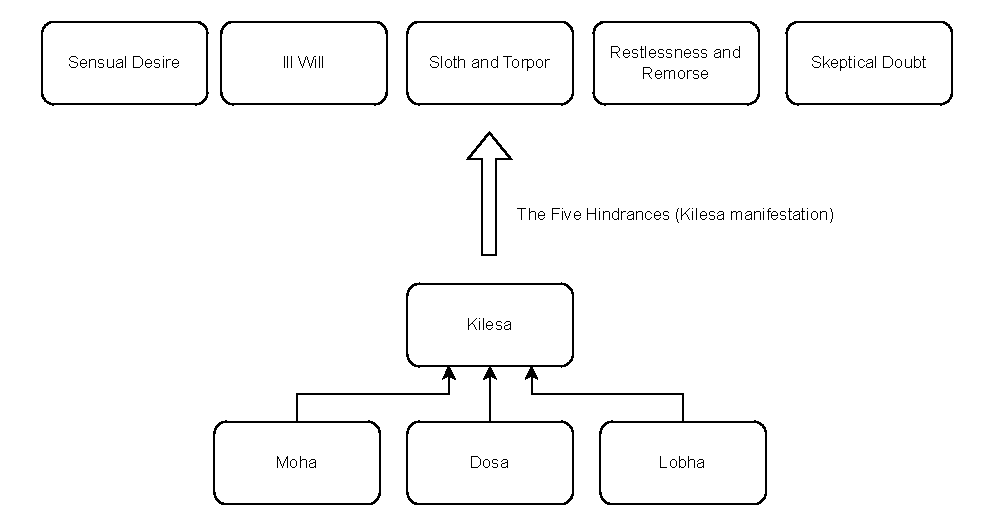
\includegraphics[width=0.75\textwidth]{kilesas.pdf}
	\end{figure}
	

	The Third Noble Truth, the truth of the cessation of suffering - Dukkha (Nirodha), illustrates that suffering can be ended by a complete uprooting of the three poisons of Kilesa, which are Moha, Dosa, and Lobha. Indeed, the third noble truth can be considered as a connecting bridge between the second and forth noble truth, while the first noble truth leads the way. It also emphasizes hope, showing that cessation of suffering is possible.
	
	The truth of the path leading to the cessation of suffering (Magga Sacca) is the Fourth Noble Truth, also known as the Noble Eightfold Path. It is often divided into three components: wisdom comprises right view and right intention. Morality comprises right action, right speech, right livelihood. Whereas concentration comprises right effort, right mindfulness, and right concentration (Figure 2). The Eightfold Path is also considered to be the core principle in the middle way, which represents a path balancing between extreme asceticism and sensual-indulgence, in which Gautama had experienced both, encouraging one to avoid both extremes. These extremes can drive Kilesa such as Lobha and Moha, preventing one from being liberated. \cite{sumedho1992four}
	
	\begin{figure}[h]
		\caption{The Fourth Noble Truth (The Eightfold Path)}
		\centering
		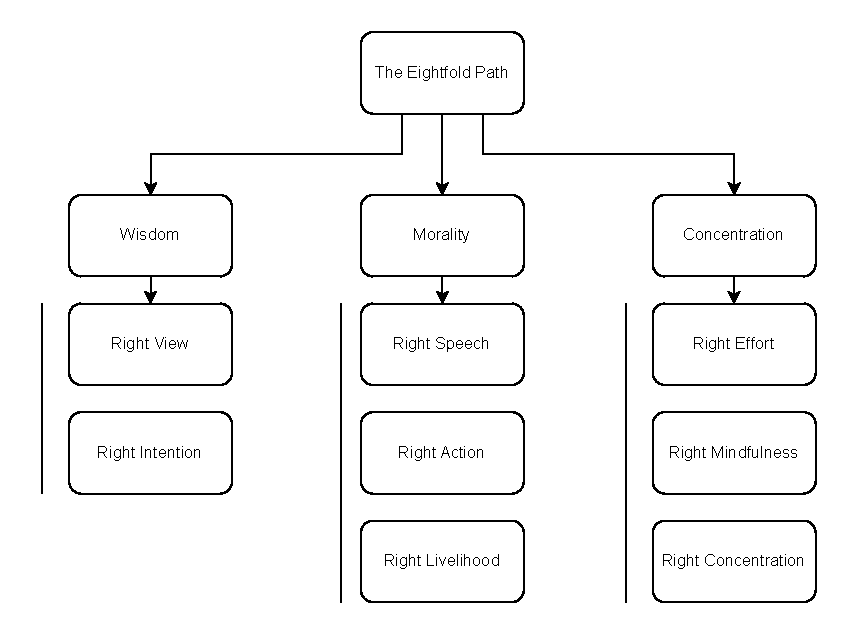
\includegraphics[width=0.75\textwidth]{TheEightfoldPath.pdf}
	\end{figure}
	
	Meditation have been around for centuries, during the Vedic period, its original purpose is to achieve spiritual liberation. For hundred of years, meditation has been evolved over time, many techniques of it were adopted. Modern-day meditation is to improve focus, mental well-being, managing stress \cite{sharma2015meditation}.  In buddhism, meditation is a really effective way to maintain mindfulness, and concentration, not to be controlled by Kilesa. Classically, meditation has two main techniques: Samatha and Vipassana, Samatha usually focuses on a single point, such as breath, whereas Vipassana involves observing the whole field of consciousness, such as thought, emotion. Despite their differences, both techniques are practiced together, where Samatha provides the base for Vipassana \cite{dhammiko2024samatha}. 
	
	For me, the Four Noble Truths can be shorten to just a sentence, for systematic resolution of urgent in any situation:
	
	"suffering exists (the First Noble Truth), it comes from Kilesa (the Second Noble Truth), ending it is possible (the Third Noble Truth) through the Eightfold Path (the Fourth Noble Truth)".
	
	\noindent A useful analogy of meditation is that; it transforms our mental concentration from a flash of light to a laser.
	
	\section{Application of The Four Noble Truths}
	Apparently, these truths could be regarded as concise axioms for logical derivation of many great philosophical statements. Indeed, every question of suffering can be answered from them. In any case, neither one of these components can be dropped out (The Eightfold Path) because there is a really tight connection in them. However, despite its subtlety and simplicity, applying them effectively requires direct experience (Observe it with the application of the four noble truths), consistency, and feedback.

	Many misuses of them can arise due to conceptual misunderstanding, ignorance of both extremes - middle way, and weak part in applying the Four Noble Truths. Take for example the problem underestimation, this can be resulting from a little sense of ego, believing that one is fully free from Kilesa, for instance distraction such as stimulation. Even the tree (Kilesa) is small, it is not yet completely uprooted; small feet such as stimulation can water the tree, further weakening our right concentration (mental muscle). 
	
	\subsection{Management of Fatigue and Pulse of Kilesa}
	
	Mental fatigue can sometimes arise due to Kilesa, as pointed out by both Gautama and ancient yogis. For instance, clinging to the difficulty of problems or situation, not getting something one wants. It is the third manifestation of Kilesa, sloth and torpor. While physical fatigue is also giving rise to mental fatigue, mental fatigue itself is what causes suffering. This difficulty can be resolved by accepting that mental fatigue exists\footnote{First Noble Truth}, it comes from Moha, Dosa, Lobha, i.e., craving and clinging\footnote{Second Noble Truth}, it can be ended with the application of the Eightfold Path\footnote{Third Noble Truth}.
	
	Another problem is to manage big pulse of Kilesa, dopamine, such as being ego to be great, self punishment of failure - reacting instead of observing, lack of patient, craving for stimulation and quick relieve, boredom, urgent. To calm the pulse, the Four Noble Truths can be applied as follow: 1) Believe that it exists, and it is just a pulse - observe it instead of react to it, 2) It comes from Kilesa (Moha, Dosa, and Lobha), 3) It can be ended. 4) Use these three points to see the truth, intent to calm it, and calm it by being mindful with effort - mostly this works through consistent meditation to maintain concentration, or as a slogan, to build mental muscle. (Figure 3) shows how The Four Truths can weaken the strength of Kilesa each time it appears, Whereas (Figure 4) shows the accumulated strength of Kilesa each time The Four Noble Truths are not being applied, and hence bad habits.
	
	\begin{figure}[H]
		\centering
		\definecolor{qqwuqq}{rgb}{0.,0.39215686274509803,0.}
\begin{tikzpicture}[line cap=round,line join=round,>=triangle 45,x=0.1cm,y=0.1cm]
	\begin{axis}[
		xlabel={Frequency},
		ylabel={Strength of Kilesa},
		x=0.1cm,y=0.1cm,
		axis lines=middle,
		ticks=none,
		xmin=0.0,
		xmax=88.0,
		ymin=0.0,
		ymax=30.0,
		]
		\clip(0.,0.) rectangle (88.,30.);
		\draw[line width=4.pt] (-5.202387737278972,44.71476789172267) -- (31.530953703318307,44.71476789172267);
		\draw[line width=4.pt] (35.57162126178401,45.08210130612865) -- (72.30496270238129,45.08210130612865);
		\draw[line width=4.pt] (8.02161518133605,34.613098995558424) -- (44.75495662193333,34.613098995558424);
		\draw[line width=2.pt,color=qqwuqq] (0.0,0.0) -- (0.0,0.0);
		\draw[line width=2.pt,color=qqwuqq] (0.0,0.0) -- (0.22,-7.697138572850605);
		\draw[line width=2.pt,color=qqwuqq] (0.22,-7.697138572850605) -- (0.44,-14.765072003761265);
		\draw[line width=2.pt,color=qqwuqq] (0.44,-14.765072003761265) -- (0.66,-20.95736108785626);
		\draw[line width=2.pt,color=qqwuqq] (0.66,-20.95736108785626) -- (0.88,-26.072061666106716);
		\draw[line width=2.pt,color=qqwuqq] (0.88,-26.072061666106716) -- (1.1,-29.957624385001246);
		\draw[line width=2.pt,color=qqwuqq] (1.1,-29.957624385001246) -- (1.32,-32.5165902517844);
		\draw[line width=2.pt,color=qqwuqq] (1.32,-32.5165902517844) -- (1.54,-33.70703385218185);
		\draw[line width=2.pt,color=qqwuqq] (1.54,-33.70703385218185) -- (1.76,-33.54179533332924);
		\draw[line width=2.pt,color=qqwuqq] (1.76,-33.54179533332924) -- (1.98,-32.08562605852601);
		\draw[line width=2.pt,color=qqwuqq] (1.98,-32.08562605852601) -- (2.2,-29.450448203116483);
		\draw[line width=2.pt,color=qqwuqq] (2.2,-29.450448203116483) -- (2.4200000000000004,-25.78899292913581);
		\draw[line width=2.pt,color=qqwuqq] (2.4200000000000004,-25.78899292913581) -- (2.6400000000000006,-21.287133132604232);
		\draw[line width=2.pt,color=qqwuqq] (2.6400000000000006,-21.287133132604232) -- (2.8600000000000008,-16.155263674176727);
		\draw[line width=2.pt,color=qqwuqq] (2.8600000000000008,-16.155263674176727) -- (3.080000000000001,-10.619103674162359);
		\draw[line width=2.pt,color=qqwuqq] (3.080000000000001,-10.619103674162359) -- (3.300000000000001,-4.910301694395456);
		\draw[line width=2.pt,color=qqwuqq] (3.300000000000001,-4.910301694395456) -- (3.5200000000000014,0.742784135321981);
		\draw[line width=2.pt,color=qqwuqq] (3.5200000000000014,0.742784135321981) -- (3.7400000000000015,6.123781774329325);
		\draw[line width=2.pt,color=qqwuqq] (3.7400000000000015,6.123781774329325) -- (3.9600000000000017,11.036162761467084);
		\draw[line width=2.pt,color=qqwuqq] (3.9600000000000017,11.036162761467084) -- (4.1800000000000015,15.309993539160846);
		\draw[line width=2.pt,color=qqwuqq] (4.1800000000000015,15.309993539160846) -- (4.400000000000001,18.807366955870705);
		\draw[line width=2.pt,color=qqwuqq] (4.400000000000001,18.807366955870705) -- (4.620000000000001,21.4263605647227);
		\draw[line width=2.pt,color=qqwuqq] (4.620000000000001,21.4263605647227) -- (4.840000000000001,23.103431950575466);
		\draw[line width=2.pt,color=qqwuqq] (4.840000000000001,23.103431950575466) -- (5.0600000000000005,23.81422566780873);
		\draw[line width=2.pt,color=qqwuqq] (5.0600000000000005,23.81422566780873) -- (5.28,23.572828934787616);
		\draw[line width=2.pt,color=qqwuqq] (5.28,23.572828934787616) -- (5.5,22.42957166398374);
		\draw[line width=2.pt,color=qqwuqq] (5.5,22.42957166398374) -- (5.72,20.467518625611778);
		\draw[line width=2.pt,color=qqwuqq] (5.72,20.467518625611778) -- (5.9399999999999995,17.79784579402967);
		\draw[line width=2.pt,color=qqwuqq] (5.9399999999999995,17.79784579402967) -- (6.159999999999999,14.55432784052431);
		\draw[line width=2.pt,color=qqwuqq] (6.159999999999999,14.55432784052431) -- (6.379999999999999,10.887188364221014);
		\draw[line width=2.pt,color=qqwuqq] (6.379999999999999,10.887188364221014) -- (6.599999999999999,6.9565782844080015);
		\draw[line width=2.pt,color=qqwuqq] (6.599999999999999,6.9565782844080015) -- (6.8199999999999985,2.9259507820335067);
		\draw[line width=2.pt,color=qqwuqq] (6.8199999999999985,2.9259507820335067) -- (7.039999999999998,-1.0444063714242855);
		\draw[line width=2.pt,color=qqwuqq] (7.039999999999998,-1.0444063714242855) -- (7.259999999999998,-4.80343757834607);
		\draw[line width=2.pt,color=qqwuqq] (7.259999999999998,-4.80343757834607) -- (7.479999999999998,-8.21476775060097);
		\draw[line width=2.pt,color=qqwuqq] (7.479999999999998,-8.21476775060097) -- (7.6999999999999975,-11.161347990614303);
		\draw[line width=2.pt,color=qqwuqq] (7.6999999999999975,-11.161347990614303) -- (7.919999999999997,-13.549153384423365);
		\draw[line width=2.pt,color=qqwuqq] (7.919999999999997,-13.549153384423365) -- (8.139999999999997,-15.309830607587696);
		\draw[line width=2.pt,color=qqwuqq] (8.139999999999997,-15.309830607587696) -- (8.359999999999998,-16.402238089889128);
		\draw[line width=2.pt,color=qqwuqq] (8.359999999999998,-16.402238089889128) -- (8.579999999999998,-16.81286680650473);
		\draw[line width=2.pt,color=qqwuqq] (8.579999999999998,-16.81286680650473) -- (8.799999999999999,-16.555173595933898);
		\draw[line width=2.pt,color=qqwuqq] (8.799999999999999,-16.555173595933898) -- (9.02,-15.667899616221296);
		\draw[line width=2.pt,color=qqwuqq] (9.02,-15.667899616221296) -- (9.24,-14.212482699803692);
		\draw[line width=2.pt,color=qqwuqq] (9.24,-14.212482699803692) -- (9.46,-12.269702751085836);
		\draw[line width=2.pt,color=qqwuqq] (9.46,-12.269702751085836) -- (9.680000000000001,-9.935723021948352);
		\draw[line width=2.pt,color=qqwuqq] (9.680000000000001,-9.935723021948352) -- (9.900000000000002,-7.317706470073673);
		\draw[line width=2.pt,color=qqwuqq] (9.900000000000002,-7.317706470073673) -- (10.120000000000003,-4.52919513490777);
		\draw[line width=2.pt,color=qqwuqq] (10.120000000000003,-4.52919513490777) -- (10.340000000000003,-1.6854415472740847);
		\draw[line width=2.pt,color=qqwuqq] (10.340000000000003,-1.6854415472740847) -- (10.560000000000004,1.101125091471835);
		\draw[line width=2.pt,color=qqwuqq] (10.560000000000004,1.101125091471835) -- (10.780000000000005,3.725128306400701);
		\draw[line width=2.pt,color=qqwuqq] (10.780000000000005,3.725128306400701) -- (11.000000000000005,6.092018751670486);
		\draw[line width=2.pt,color=qqwuqq] (11.000000000000005,6.092018751670486) -- (11.220000000000006,8.12126713789614);
		\draw[line width=2.pt,color=qqwuqq] (11.220000000000006,8.12126713789614) -- (11.440000000000007,9.748877150419677);
		\draw[line width=2.pt,color=qqwuqq] (11.440000000000007,9.748877150419677) -- (11.660000000000007,10.92915038203203);
		\draw[line width=2.pt,color=qqwuqq] (11.660000000000007,10.92915038203203) -- (11.880000000000008,11.635667176323414);
		\draw[line width=2.pt,color=qqwuqq] (11.880000000000008,11.635667176323414) -- (12.100000000000009,11.86147917566661);
		\draw[line width=2.pt,color=qqwuqq] (12.100000000000009,11.86147917566661) -- (12.32000000000001,11.618540055359144);
		\draw[line width=2.pt,color=qqwuqq] (12.32000000000001,11.618540055359144) -- (12.54000000000001,10.936429267179138);
		\draw[line width=2.pt,color=qqwuqq] (12.54000000000001,10.936429267179138) -- (12.76000000000001,9.860448615718127);
		\draw[line width=2.pt,color=qqwuqq] (12.76000000000001,9.860448615718127) -- (12.980000000000011,8.449192325699865);
		\draw[line width=2.pt,color=qqwuqq] (12.980000000000011,8.449192325699865) -- (13.200000000000012,6.771707301080872);
		\draw[line width=2.pt,color=qqwuqq] (13.200000000000012,6.771707301080872) -- (13.420000000000012,4.9043711125072695);
		\draw[line width=2.pt,color=qqwuqq] (13.420000000000012,4.9043711125072695) -- (13.640000000000013,2.927620683470099);
		\draw[line width=2.pt,color=qqwuqq] (13.640000000000013,2.927620683470099) -- (13.860000000000014,0.9226646995078489);
		\draw[line width=2.pt,color=qqwuqq] (13.860000000000014,0.9226646995078489) -- (14.080000000000014,-1.0316923314599729);
		\draw[line width=2.pt,color=qqwuqq] (14.080000000000014,-1.0316923314599729) -- (14.300000000000015,-2.8619962672016284);
		\draw[line width=2.pt,color=qqwuqq] (14.300000000000015,-2.8619962672016284) -- (14.520000000000016,-4.502755642158769);
		\draw[line width=2.pt,color=qqwuqq] (14.520000000000016,-4.502755642158769) -- (14.740000000000016,-5.8986333788590795);
		\draw[line width=2.pt,color=qqwuqq] (14.740000000000016,-5.8986333788590795) -- (14.960000000000017,-7.006151187230379);
		\draw[line width=2.pt,color=qqwuqq] (14.960000000000017,-7.006151187230379) -- (15.180000000000017,-7.794861669632455);
		\draw[line width=2.pt,color=qqwuqq] (15.180000000000017,-7.794861669632455) -- (15.400000000000018,-8.247965685137913);
		\draw[line width=2.pt,color=qqwuqq] (15.400000000000018,-8.247965685137913) -- (15.620000000000019,-8.362374960897561);
		\draw[line width=2.pt,color=qqwuqq] (15.620000000000019,-8.362374960897561) -- (15.84000000000002,-8.148241407492508);
		\draw[line width=2.pt,color=qqwuqq] (15.84000000000002,-8.148241407492508) -- (16.06000000000002,-7.6279943097169935);
		\draw[line width=2.pt,color=qqwuqq] (16.06000000000002,-7.6279943097169935) -- (16.28000000000002,-6.834943836838869);
		\draw[line width=2.pt,color=qqwuqq] (16.28000000000002,-6.834943836838869) -- (16.500000000000018,-5.811523583727534);
		\draw[line width=2.pt,color=qqwuqq] (16.500000000000018,-5.811523583727534) -- (16.720000000000017,-4.607255693550144);
		\draw[line width=2.pt,color=qqwuqq] (16.720000000000017,-4.607255693550144) -- (16.940000000000015,-3.2765292521059783);
		\draw[line width=2.pt,color=qqwuqq] (16.940000000000015,-3.2765292521059783) -- (17.160000000000014,-1.876285966274783);
		\draw[line width=2.pt,color=qqwuqq] (17.160000000000014,-1.876285966274783) -- (17.380000000000013,-0.46370668022907297);
		\draw[line width=2.pt,color=qqwuqq] (17.380000000000013,-0.46370668022907297) -- (17.600000000000012,0.9060117764752263);
		\draw[line width=2.pt,color=qqwuqq] (17.600000000000012,0.9060117764752263) -- (17.82000000000001,2.1817072629621226);
		\draw[line width=2.pt,color=qqwuqq] (17.82000000000001,2.1817072629621226) -- (18.04000000000001,3.31805858811396);
		\draw[line width=2.pt,color=qqwuqq] (18.04000000000001,3.31805858811396) -- (18.26000000000001,4.277087978657968);
		\draw[line width=2.pt,color=qqwuqq] (18.26000000000001,4.277087978657968) -- (18.480000000000008,5.029314686900375);
		\draw[line width=2.pt,color=qqwuqq] (18.480000000000008,5.029314686900375) -- (18.700000000000006,5.554530111367389);
		\draw[line width=2.pt,color=qqwuqq] (18.700000000000006,5.554530111367389) -- (18.920000000000005,5.84218072610686);
		\draw[line width=2.pt,color=qqwuqq] (18.920000000000005,5.84218072610686) -- (19.140000000000004,5.891360881844056);
		\draw[line width=2.pt,color=qqwuqq] (19.140000000000004,5.891360881844056) -- (19.360000000000003,5.710432551054702);
		\draw[line width=2.pt,color=qqwuqq] (19.360000000000003,5.710432551054702) -- (19.580000000000002,5.316302791138203);
		\draw[line width=2.pt,color=qqwuqq] (19.580000000000002,5.316302791138203) -- (19.8,4.733401621233746);
		\draw[line width=2.pt,color=qqwuqq] (19.8,4.733401621233746) -- (20.02,3.992412764126272);
		\draw[line width=2.pt,color=qqwuqq] (20.02,3.992412764126272) -- (20.24,3.128817010807807);
		\draw[line width=2.pt,color=qqwuqq] (20.24,3.128817010807807) -- (20.459999999999997,2.181312644302326);
		\draw[line width=2.pt,color=qqwuqq] (20.459999999999997,2.181312644302326) -- (20.679999999999996,1.190179343341063);
		\draw[line width=2.pt,color=qqwuqq] (20.679999999999996,1.190179343341063) -- (20.899999999999995,0.19565131462067983);
		\draw[line width=2.pt,color=qqwuqq] (20.899999999999995,0.19565131462067983) -- (21.119999999999994,-0.7636377849851956);
		\draw[line width=2.pt,color=qqwuqq] (21.119999999999994,-0.7636377849851956) -- (21.339999999999993,-1.6520810461300006);
		\draw[line width=2.pt,color=qqwuqq] (21.339999999999993,-1.6520810461300006) -- (21.55999999999999,-2.438345979555202);
		\draw[line width=2.pt,color=qqwuqq] (21.55999999999999,-2.438345979555202) -- (21.77999999999999,-3.0964030642680007);
		\draw[line width=2.pt,color=qqwuqq] (21.77999999999999,-3.0964030642680007) -- (21.99999999999999,-3.606304799690853);
		\draw[line width=2.pt,color=qqwuqq] (21.99999999999999,-3.606304799690853) -- (22.219999999999988,-3.95469585283523);
		\draw[line width=2.pt,color=qqwuqq] (22.219999999999988,-3.95469585283523) -- (22.439999999999987,-4.135046133461846);
		\draw[line width=2.pt,color=qqwuqq] (22.439999999999987,-4.135046133461846) -- (22.659999999999986,-4.1476097042383);
		\draw[line width=2.pt,color=qqwuqq] (22.659999999999986,-4.1476097042383) -- (22.879999999999985,-3.9991229177599967);
		\draw[line width=2.pt,color=qqwuqq] (22.879999999999985,-3.9991229177599967) -- (23.099999999999984,-3.702264687568559);
		\draw[line width=2.pt,color=qqwuqq] (23.099999999999984,-3.702264687568559) -- (23.319999999999983,-3.2749100194853726);
		\draw[line width=2.pt,color=qqwuqq] (23.319999999999983,-3.2749100194853726) -- (23.53999999999998,-2.7392145903920353);
		\draw[line width=2.pt,color=qqwuqq] (23.53999999999998,-2.7392145903920353) -- (23.75999999999998,-2.1205730733463835);
		\draw[line width=2.pt,color=qqwuqq] (23.75999999999998,-2.1205730733463835) -- (23.97999999999998,-1.4464969558319472);
		\draw[line width=2.pt,color=qqwuqq] (23.97999999999998,-1.4464969558319472) -- (24.199999999999978,-0.7454587442781538);
		\draw[line width=2.pt,color=qqwuqq] (24.199999999999978,-0.7454587442781538) -- (24.419999999999977,-0.0457487302522797);
		\draw[line width=2.pt,color=qqwuqq] (24.419999999999977,-0.0457487302522797) -- (24.639999999999976,0.6256119800718075);
		\draw[line width=2.pt,color=qqwuqq] (24.639999999999976,0.6256119800718075) -- (24.859999999999975,1.2438625300934443);
		\draw[line width=2.pt,color=qqwuqq] (24.859999999999975,1.2438625300934443) -- (25.079999999999973,1.7873632455232529);
		\draw[line width=2.pt,color=qqwuqq] (25.079999999999973,1.7873632455232529) -- (25.299999999999972,2.238298719838817);
		\draw[line width=2.pt,color=qqwuqq] (25.299999999999972,2.238298719838817) -- (25.51999999999997,2.5832026382516364);
		\draw[line width=2.pt,color=qqwuqq] (25.51999999999997,2.5832026382516364) -- (25.73999999999997,2.8132917033227165);
		\draw[line width=2.pt,color=qqwuqq] (25.73999999999997,2.8132917033227165) -- (25.95999999999997,2.924603956961746);
		\draw[line width=2.pt,color=qqwuqq] (25.95999999999997,2.924603956961746) -- (26.179999999999968,2.917944565808271);
		\draw[line width=2.pt,color=qqwuqq] (26.179999999999968,2.917944565808271) -- (26.399999999999967,2.798649456001648);
		\draw[line width=2.pt,color=qqwuqq] (26.399999999999967,2.798649456001648) -- (26.619999999999965,2.576183785368919);
		\draw[line width=2.pt,color=qqwuqq] (26.619999999999965,2.576183785368919) -- (26.839999999999964,2.263597901466886);
		\draw[line width=2.pt,color=qqwuqq] (26.839999999999964,2.263597901466886) -- (27.059999999999963,1.8768679741851166);
		\draw[line width=2.pt,color=qqwuqq] (27.059999999999963,1.8768679741851166) -- (27.279999999999962,1.4341517842629454);
		\draw[line width=2.pt,color=qqwuqq] (27.279999999999962,1.4341517842629454) -- (27.49999999999996,0.9549921203775262);
		\draw[line width=2.pt,color=qqwuqq] (27.49999999999996,0.9549921203775262) -- (27.71999999999996,0.4595008680127001);
		\draw[line width=2.pt,color=qqwuqq] (27.71999999999996,0.4595008680127001) -- (27.93999999999996,-0.032443803568422684);
		\draw[line width=2.pt,color=qqwuqq] (27.93999999999996,-0.032443803568422684) -- (28.159999999999958,-0.5019566517757769);
		\draw[line width=2.pt,color=qqwuqq] (28.159999999999958,-0.5019566517757769) -- (28.379999999999956,-0.931833464583169);
		\draw[line width=2.pt,color=qqwuqq] (28.379999999999956,-0.931833464583169) -- (28.599999999999955,-1.3071444895827784);
		\draw[line width=2.pt,color=qqwuqq] (28.599999999999955,-1.3071444895827784) -- (28.819999999999954,-1.615714298297988);
		\draw[line width=2.pt,color=qqwuqq] (28.819999999999954,-1.615714298297988) -- (29.039999999999953,-1.8484744038596068);
		\draw[line width=2.pt,color=qqwuqq] (29.039999999999953,-1.8484744038596068) -- (29.259999999999952,-1.9996804634565513);
		\draw[line width=2.pt,color=qqwuqq] (29.259999999999952,-1.9996804634565513) -- (29.47999999999995,-2.066991489070003);
		\draw[line width=2.pt,color=qqwuqq] (29.47999999999995,-2.066991489070003) -- (29.69999999999995,-2.051413941089435);
		\draw[line width=2.pt,color=qqwuqq] (29.69999999999995,-2.051413941089435) -- (29.91999999999995,-1.957118684604914);
		\draw[line width=2.pt,color=qqwuqq] (29.91999999999995,-1.957118684604914) -- (30.139999999999947,-1.791143364795643);
		\draw[line width=2.pt,color=qqwuqq] (30.139999999999947,-1.791143364795643) -- (30.359999999999946,-1.5629966515299445);
		\draw[line width=2.pt,color=qqwuqq] (30.359999999999946,-1.5629966515299445) -- (30.579999999999945,-1.2841838927712768);
		\draw[line width=2.pt,color=qqwuqq] (30.579999999999945,-1.2841838927712768) -- (30.799999999999944,-0.9676759167058999);
		\draw[line width=2.pt,color=qqwuqq] (30.799999999999944,-0.9676759167058999) -- (31.019999999999943,-0.6273439867945376);
		\draw[line width=2.pt,color=qqwuqq] (31.019999999999943,-0.6273439867945376) -- (31.23999999999994,-0.27738423356835124);
		\draw[line width=2.pt,color=qqwuqq] (31.23999999999994,-0.27738423356835124) -- (31.45999999999994,0.06824570976631764);
		\draw[line width=2.pt,color=qqwuqq] (31.45999999999994,0.06824570976631764) -- (31.67999999999994,0.39635659143858176);
		\draw[line width=2.pt,color=qqwuqq] (31.67999999999994,0.39635659143858176) -- (31.899999999999938,0.6950048799947598);
		\draw[line width=2.pt,color=qqwuqq] (31.899999999999938,0.6950048799947598) -- (32.11999999999994,0.9539013471401625);
		\draw[line width=2.pt,color=qqwuqq] (32.11999999999994,0.9539013471401625) -- (32.33999999999994,1.164738042350916);
		\draw[line width=2.pt,color=qqwuqq] (32.33999999999994,1.164738042350916) -- (32.55999999999994,1.3214245184824622);
		\draw[line width=2.pt,color=qqwuqq] (32.55999999999994,1.3214245184824622) -- (32.77999999999994,1.420228072996944);
		\draw[line width=2.pt,color=qqwuqq] (32.77999999999994,1.420228072996944) -- (32.999999999999936,1.4598167093216667);
		\draw[line width=2.pt,color=qqwuqq] (32.999999999999936,1.4598167093216667) -- (33.219999999999935,1.4412073432779031);
		\draw[line width=2.pt,color=qqwuqq] (33.219999999999935,1.4412073432779031) -- (33.439999999999934,1.3676253377791667);
		\draw[line width=2.pt,color=qqwuqq] (33.439999999999934,1.3676253377791667) -- (33.65999999999993,1.244284618673285);
		\draw[line width=2.pt,color=qqwuqq] (33.65999999999993,1.244284618673285) -- (33.87999999999993,1.078100299756258);
		\draw[line width=2.pt,color=qqwuqq] (33.87999999999993,1.078100299756258) -- (34.09999999999993,0.8773478433784867);
		\draw[line width=2.pt,color=qqwuqq] (34.09999999999993,0.8773478433784867) -- (34.31999999999993,0.6512842483166236);
		\draw[line width=2.pt,color=qqwuqq] (34.31999999999993,0.6512842483166236) -- (34.53999999999993,0.4097475592469367);
		\draw[line width=2.pt,color=qqwuqq] (34.53999999999993,0.4097475592469367) -- (34.75999999999993,0.1627511296878543);
		\draw[line width=2.pt,color=qqwuqq] (34.75999999999993,0.1627511296878543) -- (34.979999999999926,-0.07991143401028794);
		\draw[line width=2.pt,color=qqwuqq] (34.979999999999926,-0.07991143401028794) -- (35.199999999999925,-0.3090358190186316);
		\draw[line width=2.pt,color=qqwuqq] (35.199999999999925,-0.3090358190186316) -- (35.41999999999992,-0.516337839635034);
		\draw[line width=2.pt,color=qqwuqq] (35.41999999999992,-0.516337839635034) -- (35.63999999999992,-0.6947344215465338);
		\draw[line width=2.pt,color=qqwuqq] (35.63999999999992,-0.6947344215465338) -- (35.85999999999992,-0.8385660086749794);
		\draw[line width=2.pt,color=qqwuqq] (35.85999999999992,-0.8385660086749794) -- (36.07999999999992,-0.9437543071449703);
		\draw[line width=2.pt,color=qqwuqq] (36.07999999999992,-0.9437543071449703) -- (36.29999999999992,-1.0078920452758267);
		\draw[line width=2.pt,color=qqwuqq] (36.29999999999992,-1.0078920452758267) -- (36.51999999999992,-1.0302642023908146);
		\draw[line width=2.pt,color=qqwuqq] (36.51999999999992,-1.0302642023908146) -- (36.73999999999992,-1.0118028349000505);
		\draw[line width=2.pt,color=qqwuqq] (36.73999999999992,-1.0118028349000505) -- (36.959999999999916,-0.9549801062300836);
		\draw[line width=2.pt,color=qqwuqq] (36.959999999999916,-0.9549801062300836) -- (37.179999999999914,-0.863646320345689);
		\draw[line width=2.pt,color=qqwuqq] (37.179999999999914,-0.863646320345689) -- (37.39999999999991,-0.7428215942290297);
		\draw[line width=2.pt,color=qqwuqq] (37.39999999999991,-0.7428215942290297) -- (37.61999999999991,-0.5984512271024954);
		\draw[line width=2.pt,color=qqwuqq] (37.61999999999991,-0.5984512271024954) -- (37.83999999999991,-0.43713579614376397);
		\draw[line width=2.pt,color=qqwuqq] (37.83999999999991,-0.43713579614376397) -- (38.05999999999991,-0.26584751172147936);
		\draw[line width=2.pt,color=qqwuqq] (38.05999999999991,-0.26584751172147936) -- (38.27999999999991,-0.09164440047534003);
		\draw[line width=2.pt,color=qqwuqq] (38.27999999999991,-0.09164440047534003) -- (38.49999999999991,0.07860652934515276);
		\draw[line width=2.pt,color=qqwuqq] (38.49999999999991,0.07860652934515276) -- (38.71999999999991,0.23848681362951732);
		\draw[line width=2.pt,color=qqwuqq] (38.71999999999991,0.23848681362951732) -- (38.939999999999905,0.38225561435168864);
		\draw[line width=2.pt,color=qqwuqq] (38.939999999999905,0.38225561435168864) -- (39.159999999999904,0.5050427167967401);
		\draw[line width=2.pt,color=qqwuqq] (39.159999999999904,0.5050427167967401) -- (39.3799999999999,0.6029995265179889);
		\draw[line width=2.pt,color=qqwuqq] (39.3799999999999,0.6029995265179889) -- (39.5999999999999,0.6734040304949607);
		\draw[line width=2.pt,color=qqwuqq] (39.5999999999999,0.6734040304949607) -- (39.8199999999999,0.7147176422290581);
		\draw[line width=2.pt,color=qqwuqq] (39.8199999999999,0.7147176422290581) -- (40.0399999999999,0.7265938021182425);
		\draw[line width=2.pt,color=qqwuqq] (40.0399999999999,0.7265938021182425) -- (40.2599999999999,0.7098400770266174);
		\draw[line width=2.pt,color=qqwuqq] (40.2599999999999,0.7098400770266174) -- (40.4799999999999,0.6663372274443005);
		\draw[line width=2.pt,color=qqwuqq] (40.4799999999999,0.6663372274443005) -- (40.699999999999896,0.5989202266558197);
		\draw[line width=2.pt,color=qqwuqq] (40.699999999999896,0.5989202266558197) -- (40.919999999999895,0.5112274742060655);
		\draw[line width=2.pt,color=qqwuqq] (40.919999999999895,0.5112274742060655) -- (41.139999999999894,0.4075254081050115);
		\draw[line width=2.pt,color=qqwuqq] (41.139999999999894,0.4075254081050115) -- (41.35999999999989,0.29251636214109067);
		\draw[line width=2.pt,color=qqwuqq] (41.35999999999989,0.29251636214109067) -- (41.57999999999989,0.17113782532025057);
		\draw[line width=2.pt,color=qqwuqq] (41.57999999999989,0.17113782532025057) -- (41.79999999999989,0.04836124205209212);
		\draw[line width=2.pt,color=qqwuqq] (41.79999999999989,0.04836124205209212) -- (42.01999999999989,-0.07100184085821072);
		\draw[line width=2.pt,color=qqwuqq] (42.01999999999989,-0.07100184085821072) -- (42.23999999999989,-0.182479094689631);
		\draw[line width=2.pt,color=qqwuqq] (42.23999999999989,-0.182479094689631) -- (42.45999999999989,-0.2820958827494091);
		\draw[line width=2.pt,color=qqwuqq] (42.45999999999989,-0.2820958827494091) -- (42.679999999999886,-0.36650765231360444);
		\draw[line width=2.pt,color=qqwuqq] (42.679999999999886,-0.36650765231360444) -- (42.899999999999885,-0.4331022438171245);
		\draw[line width=2.pt,color=qqwuqq] (42.899999999999885,-0.4331022438171245) -- (43.119999999999884,-0.4800694529437324);
		\draw[line width=2.pt,color=qqwuqq] (43.119999999999884,-0.4800694529437324) -- (43.33999999999988,-0.5064365632457033);
		\draw[line width=2.pt,color=qqwuqq] (43.33999999999988,-0.5064365632457033) -- (43.55999999999988,-0.5120699390400145);
		\draw[line width=2.pt,color=qqwuqq] (43.55999999999988,-0.5120699390400145) -- (43.77999999999988,-0.49764407790795095);
		\draw[line width=2.pt,color=qqwuqq] (43.77999999999988,-0.49764407790795095) -- (43.99999999999988,-0.46458072117962945);
		\draw[line width=2.pt,color=qqwuqq] (43.99999999999988,-0.46458072117962945) -- (44.21999999999988,-0.4149616676696555);
		\draw[line width=2.pt,color=qqwuqq] (44.21999999999988,-0.4149616676696555) -- (44.43999999999988,-0.3514197966812836);
		\draw[line width=2.pt,color=qqwuqq] (44.43999999999988,-0.3514197966812836) -- (44.659999999999876,-0.2770134556160711);
		\draw[line width=2.pt,color=qqwuqq] (44.659999999999876,-0.2770134556160711) -- (44.879999999999875,-0.19508978938706306);
		\draw[line width=2.pt,color=qqwuqq] (44.879999999999875,-0.19508978938706306) -- (45.09999999999987,-0.10914277670160633);
		\draw[line width=2.pt,color=qqwuqq] (45.09999999999987,-0.10914277670160633) -- (45.31999999999987,-0.022671694956980425);
		\draw[line width=2.pt,color=qqwuqq] (45.31999999999987,-0.022671694956980425) -- (45.53999999999987,0.06095452739339439);
		\draw[line width=2.pt,color=qqwuqq] (45.53999999999987,0.06095452739339439) -- (45.75999999999987,0.13862207496850137);
		\draw[line width=2.pt,color=qqwuqq] (45.75999999999987,0.13862207496850137) -- (45.97999999999987,0.20758176629188366);
		\draw[line width=2.pt,color=qqwuqq] (45.97999999999987,0.20758176629188366) -- (46.19999999999987,0.2655397491126547);
		\draw[line width=2.pt,color=qqwuqq] (46.19999999999987,0.2655397491126547) -- (46.41999999999987,0.31072667073472127);
		\draw[line width=2.pt,color=qqwuqq] (46.41999999999987,0.31072667073472127) -- (46.639999999999866,0.34194357307740403);
		\draw[line width=2.pt,color=qqwuqq] (46.639999999999866,0.34194357307740403) -- (46.859999999999864,0.3585837382694249);
		\draw[line width=2.pt,color=qqwuqq] (46.859999999999864,0.3585837382694249) -- (47.07999999999986,0.360630674601721);
		\draw[line width=2.pt,color=qqwuqq] (47.07999999999986,0.360630674601721) -- (47.29999999999986,0.34863334784437244);
		\draw[line width=2.pt,color=qqwuqq] (47.29999999999986,0.34863334784437244) -- (47.51999999999986,0.323660595955099);
		\draw[line width=2.pt,color=qqwuqq] (47.51999999999986,0.323660595955099) -- (47.73999999999986,0.2872373873702898);
		\draw[line width=2.pt,color=qqwuqq] (47.73999999999986,0.2872373873702898) -- (47.95999999999986,0.24126617119928334);
		\draw[line width=2.pt,color=qqwuqq] (47.95999999999986,0.24126617119928334) -- (48.17999999999986,0.18793700474799527);
		\draw[line width=2.pt,color=qqwuqq] (48.17999999999986,0.18793700474799527) -- (48.39999999999986,0.1296304194643624);
		\draw[line width=2.pt,color=qqwuqq] (48.39999999999986,0.1296304194643624) -- (48.619999999999855,0.0688170969066247);
		\draw[line width=2.pt,color=qqwuqq] (48.619999999999855,0.0688170969066247) -- (48.839999999999854,0.00795837451899109);
		\draw[line width=2.pt,color=qqwuqq] (48.839999999999854,0.00795837451899109) -- (49.05999999999985,-0.050588604149497396);
		\draw[line width=2.pt,color=qqwuqq] (49.05999999999985,-0.050588604149497396) -- (49.27999999999985,-0.10465762408878401);
		\draw[line width=2.pt,color=qqwuqq] (49.27999999999985,-0.10465762408878401) -- (49.49999999999985,-0.1523490110897908);
		\draw[line width=2.pt,color=qqwuqq] (49.49999999999985,-0.1523490110897908) -- (49.71999999999985,-0.19209167425836682);
		\draw[line width=2.pt,color=qqwuqq] (49.71999999999985,-0.19209167425836682) -- (49.93999999999985,-0.2226897619039932);
		\draw[line width=2.pt,color=qqwuqq] (49.93999999999985,-0.2226897619039932) -- (50.15999999999985,-0.2433527875868393);
		\draw[line width=2.pt,color=qqwuqq] (50.15999999999985,-0.2433527875868393) -- (50.379999999999846,-0.2537087720108767);
		\draw[line width=2.pt,color=qqwuqq] (50.379999999999846,-0.2537087720108767) -- (50.599999999999845,-0.25380062328172687);
		\draw[line width=2.pt,color=qqwuqq] (50.599999999999845,-0.25380062328172687) -- (50.819999999999844,-0.24406661713275823);
		\draw[line width=2.pt,color=qqwuqq] (50.819999999999844,-0.24406661713275823) -- (51.03999999999984,-0.22530641695424475);
		\draw[line width=2.pt,color=qqwuqq] (51.03999999999984,-0.22530641695424475) -- (51.25999999999984,-0.19863457108053573);
		\draw[line width=2.pt,color=qqwuqq] (51.25999999999984,-0.19863457108053573) -- (51.47999999999984,-0.1654238260116286);
		\draw[line width=2.pt,color=qqwuqq] (51.47999999999984,-0.1654238260116286) -- (51.69999999999984,-0.12724088769087127);
		\draw[line width=2.pt,color=qqwuqq] (51.69999999999984,-0.12724088769087127) -- (51.91999999999984,-0.08577744191294598);
		\draw[line width=2.pt,color=qqwuqq] (51.91999999999984,-0.08577744191294598) -- (52.13999999999984,-0.04277930739895422);
		\draw[line width=2.pt,color=qqwuqq] (52.13999999999984,-0.04277930739895422) -- (52.359999999999836,0.0);
		\draw[line width=2.pt,color=qqwuqq] (52.359999999999836,0.0) -- (52.579999999999835,0.04098282277489705);
		\draw[line width=2.pt,color=qqwuqq] (52.579999999999835,0.04098282277489705) -- (52.799999999999834,0.07859304447723989);
		\draw[line width=2.pt,color=qqwuqq] (52.799999999999834,0.07859304447723989) -- (53.01999999999983,0.11154280006071413);
		\draw[line width=2.pt,color=qqwuqq] (53.01999999999983,0.11154280006071413) -- (53.23999999999983,0.13875757204499659);
		\draw[line width=2.pt,color=qqwuqq] (53.23999999999983,0.13875757204499659) -- (53.45999999999983,0.15943103646076215);
		\draw[line width=2.pt,color=qqwuqq] (53.45999999999983,0.15943103646076215) -- (53.67999999999983,0.17304472234446233);
		\draw[line width=2.pt,color=qqwuqq] (53.67999999999983,0.17304472234446233) -- (53.89999999999983,0.17937568526308448);
		\draw[line width=2.pt,color=qqwuqq] (53.89999999999983,0.17937568526308448) -- (54.11999999999983,0.1784924138575207);
		\draw[line width=2.pt,color=qqwuqq] (54.11999999999983,0.1784924138575207) -- (54.339999999999826,0.17073963434039147);
		\draw[line width=2.pt,color=qqwuqq] (54.339999999999826,0.17073963434039147) -- (54.559999999999825,0.15671307890256816);
		\draw[line width=2.pt,color=qqwuqq] (54.559999999999825,0.15671307890256816) -- (54.77999999999982,0.13722562648713238);
		\draw[line width=2.pt,color=qqwuqq] (54.77999999999982,0.13722562648713238) -- (54.99999999999982,0.11326649764417047);
		\draw[line width=2.pt,color=qqwuqq] (54.99999999999982,0.11326649764417047) -- (55.21999999999982,0.08595538159082872);
		\draw[line width=2.pt,color=qqwuqq] (55.21999999999982,0.08595538159082872) -- (55.43999999999982,0.05649348887528014);
		\draw[line width=2.pt,color=qqwuqq] (55.43999999999982,0.05649348887528014) -- (55.65999999999982,0.02611355621228437);
		\draw[line width=2.pt,color=qqwuqq] (55.65999999999982,0.02611355621228437) -- (55.87999999999982,-0.0039692166275070075);
		\draw[line width=2.pt,color=qqwuqq] (55.87999999999982,-0.0039692166275070075) -- (56.09999999999982,-0.032603439288229175);
		\draw[line width=2.pt,color=qqwuqq] (56.09999999999982,-0.032603439288229175) -- (56.319999999999816,-0.05874334207377909);
		\draw[line width=2.pt,color=qqwuqq] (56.319999999999816,-0.05874334207377909) -- (56.539999999999814,-0.08148469993976394);
		\draw[line width=2.pt,color=qqwuqq] (56.539999999999814,-0.08148469993976394) -- (56.75999999999981,-0.10009373242241783);
		\draw[line width=2.pt,color=qqwuqq] (56.75999999999981,-0.10009373242241783) -- (56.97999999999981,-0.11402816345593031);
		\draw[line width=2.pt,color=qqwuqq] (56.97999999999981,-0.11402816345593031) -- (57.19999999999981,-0.12294996356399919);
		\draw[line width=2.pt,color=qqwuqq] (57.19999999999981,-0.12294996356399919) -- (57.41999999999981,-0.12672963935273576);
		\draw[line width=2.pt,color=qqwuqq] (57.41999999999981,-0.12672963935273576) -- (57.63999999999981,-0.1254422681598257);
		\draw[line width=2.pt,color=qqwuqq] (57.63999999999981,-0.1254422681598257) -- (57.85999999999981,-0.11935578665455232);
		\draw[line width=2.pt,color=qqwuqq] (57.85999999999981,-0.11935578665455232) -- (58.07999999999981,-0.1089123200482965);
		\draw[line width=2.pt,color=qqwuqq] (58.07999999999981,-0.1089123200482965) -- (58.299999999999805,-0.09470357403596102);
		\draw[line width=2.pt,color=qqwuqq] (58.299999999999805,-0.09470357403596102) -- (58.519999999999804,-0.07744149735861808);
		\draw[line width=2.pt,color=qqwuqq] (58.519999999999804,-0.07744149735861808) -- (58.7399999999998,-0.05792555390637657);
		\draw[line width=2.pt,color=qqwuqq] (58.7399999999998,-0.05792555390637657) -- (58.9599999999998,-0.03700801685368983);
		\draw[line width=2.pt,color=qqwuqq] (58.9599999999998,-0.03700801685368983) -- (59.1799999999998,-0.015558713063046226);
		\draw[line width=2.pt,color=qqwuqq] (59.1799999999998,-0.015558713063046226) -- (59.3999999999998,0.00556939421267988);
		\draw[line width=2.pt,color=qqwuqq] (59.3999999999998,0.00556939421267988) -- (59.6199999999998,0.02557248848972263);
		\draw[line width=2.pt,color=qqwuqq] (59.6199999999998,0.02557248848972263) -- (59.8399999999998,0.043724891605660766);
		\draw[line width=2.pt,color=qqwuqq] (59.8399999999998,0.043724891605660766) -- (60.059999999999796,0.05940378340260204);
		\draw[line width=2.pt,color=qqwuqq] (60.059999999999796,0.05940378340260204) -- (60.279999999999795,0.07210887679423121);
		\draw[line width=2.pt,color=qqwuqq] (60.279999999999795,0.07210887679423121) -- (60.499999999999794,0.08147650395637285);
		\draw[line width=2.pt,color=qqwuqq] (60.499999999999794,0.08147650395637285) -- (60.71999999999979,0.08728780909453214);
		\draw[line width=2.pt,color=qqwuqq] (60.71999999999979,0.08728780909453214) -- (60.93999999999979,0.08947098442267719);
		\draw[line width=2.pt,color=qqwuqq] (60.93999999999979,0.08947098442267719) -- (61.15999999999979,0.08809771923865235);
		\draw[line width=2.pt,color=qqwuqq] (61.15999999999979,0.08809771923865235) -- (61.37999999999979,0.08337424861777196);
		\draw[line width=2.pt,color=qqwuqq] (61.37999999999979,0.08337424861777196) -- (61.59999999999979,0.07562758059884722);
		\draw[line width=2.pt,color=qqwuqq] (61.59999999999979,0.07562758059884722) -- (61.81999999999979,0.06528764240757072);
		\draw[line width=2.pt,color=qqwuqq] (61.81999999999979,0.06528764240757072) -- (62.039999999999786,0.052866212315003845);
		\draw[line width=2.pt,color=qqwuqq] (62.039999999999786,0.052866212315003845) -- (62.259999999999785,0.038933590818949794);
		\draw[line width=2.pt,color=qqwuqq] (62.259999999999785,0.038933590818949794) -- (62.479999999999784,0.024094011270095504);
		\draw[line width=2.pt,color=qqwuqq] (62.479999999999784,0.024094011270095504) -- (62.69999999999978,0.008960795796119013);
		\draw[line width=2.pt,color=qqwuqq] (62.69999999999978,0.008960795796119013) -- (62.91999999999978,-0.005867771064260471);
		\draw[line width=2.pt,color=qqwuqq] (62.91999999999978,-0.005867771064260471) -- (63.13999999999978,-0.01983094823866402);
		\draw[line width=2.pt,color=qqwuqq] (63.13999999999978,-0.01983094823866402) -- (63.35999999999978,-0.03242562230403283);
		\draw[line width=2.pt,color=qqwuqq] (63.35999999999978,-0.03242562230403283) -- (63.57999999999978,-0.04322329697598164);
		\draw[line width=2.pt,color=qqwuqq] (63.57999999999978,-0.04322329697598164) -- (63.79999999999978,-0.05188346363767921);
		\draw[line width=2.pt,color=qqwuqq] (63.79999999999978,-0.05188346363767921) -- (64.01999999999978,-0.05816299126022744);
		\draw[line width=2.pt,color=qqwuqq] (64.01999999999978,-0.05816299126022744) -- (64.23999999999978,-0.061921343680743535);
		\draw[line width=2.pt,color=qqwuqq] (64.23999999999978,-0.061921343680743535) -- (64.45999999999978,-0.06312160194893048);
		\draw[line width=2.pt,color=qqwuqq] (64.45999999999978,-0.06312160194893048) -- (64.67999999999978,-0.06182743275325308);
		\draw[line width=2.pt,color=qqwuqq] (64.67999999999978,-0.06182743275325308) -- (64.89999999999978,-0.05819629475169828);
		\draw[line width=2.pt,color=qqwuqq] (64.89999999999978,-0.05819629475169828) -- (65.11999999999978,-0.05246930766060665);
		\draw[line width=2.pt,color=qqwuqq] (65.11999999999978,-0.05246930766060665) -- (65.33999999999978,-0.04495831981568867);
		\draw[line width=2.pt,color=qqwuqq] (65.33999999999978,-0.04495831981568867) -- (65.55999999999977,-0.03603079527610165);
		\draw[line width=2.pt,color=qqwuqq] (65.55999999999977,-0.03603079527610165) -- (65.77999999999977,-0.026093199189950102);
		\draw[line width=2.pt,color=qqwuqq] (65.77999999999977,-0.026093199189950102) -- (65.99999999999977,-0.015573589039649728);
		\draw[line width=2.pt,color=qqwuqq] (65.99999999999977,-0.015573589039649728) -- (66.21999999999977,-0.004904119657305522);
		\draw[line width=2.pt,color=qqwuqq] (66.21999999999977,-0.004904119657305522) -- (66.43999999999977,0.005495857234578209);
		\draw[line width=2.pt,color=qqwuqq] (66.43999999999977,0.005495857234578209) -- (66.65999999999977,0.015235470513260664);
		\draw[line width=2.pt,color=qqwuqq] (66.65999999999977,0.015235470513260664) -- (66.87999999999977,0.023966230113070752);
		\draw[line width=2.pt,color=qqwuqq] (66.87999999999977,0.023966230113070752) -- (67.09999999999977,0.03139368900627338);
		\draw[line width=2.pt,color=qqwuqq] (67.09999999999977,0.03139368900627338) -- (67.31999999999977,0.037286511754685454);
		\draw[line width=2.pt,color=qqwuqq] (67.31999999999977,0.037286511754685454) -- (67.53999999999976,0.04148271032241201);
		\draw[line width=2.pt,color=qqwuqq] (67.53999999999976,0.04148271032241201) -- (67.75999999999976,0.04389292776637947);
		\draw[line width=2.pt,color=qqwuqq] (67.75999999999976,0.04389292776637947) -- (67.97999999999976,0.0445007698053615);
		\draw[line width=2.pt,color=qqwuqq] (67.97999999999976,0.0445007698053615) -- (68.19999999999976,0.04336029851315572);
		\draw[line width=2.pt,color=qqwuqq] (68.19999999999976,0.04336029851315572) -- (68.41999999999976,0.04059090728752874);
		\draw[line width=2.pt,color=qqwuqq] (68.41999999999976,0.04059090728752874) -- (68.63999999999976,0.03636988815570031);
		\draw[line width=2.pt,color=qqwuqq] (68.63999999999976,0.03636988815570031) -- (68.85999999999976,0.0309230783921366);
		\draw[line width=2.pt,color=qqwuqq] (68.85999999999976,0.0309230783921366) -- (69.07999999999976,0.02451403109589486);
		\draw[line width=2.pt,color=qqwuqq] (69.07999999999976,0.02451403109589486) -- (69.29999999999976,0.017432192356172556);
		\draw[line width=2.pt,color=qqwuqq] (69.29999999999976,0.017432192356172556) -- (69.51999999999975,0.009980585303791407);
		\draw[line width=2.pt,color=qqwuqq] (69.51999999999975,0.009980585303791407) -- (69.73999999999975,0.0024634988936706446);
		\draw[line width=2.pt,color=qqwuqq] (69.73999999999975,0.0024634988936706446) -- (69.95999999999975,-0.004825342349996366);
		\draw[line width=2.pt,color=qqwuqq] (69.95999999999975,-0.004825342349996366) -- (70.17999999999975,-0.011613690506961231);
		\draw[line width=2.pt,color=qqwuqq] (70.17999999999975,-0.011613690506961231) -- (70.39999999999975,-0.017660385578970265);
		\draw[line width=2.pt,color=qqwuqq] (70.39999999999975,-0.017660385578970265) -- (70.61999999999975,-0.022763349998141107);
		\draw[line width=2.pt,color=qqwuqq] (70.61999999999975,-0.022763349998141107) -- (70.83999999999975,-0.02676572654113785);
		\draw[line width=2.pt,color=qqwuqq] (70.83999999999975,-0.02676572654113785) -- (71.05999999999975,-0.029560002035261844);
		\draw[line width=2.pt,color=qqwuqq] (71.05999999999975,-0.029560002035261844) -- (71.27999999999975,-0.031090043975656987);
		\draw[line width=2.pt,color=qqwuqq] (71.27999999999975,-0.031090043975656987) -- (71.49999999999974,-0.0313510610789059);
		\draw[line width=2.pt,color=qqwuqq] (71.49999999999974,-0.0313510610789059) -- (71.71999999999974,-0.030387578665888565);
		\draw[line width=2.pt,color=qqwuqq] (71.71999999999974,-0.030387578665888565) -- (71.93999999999974,-0.0282895926788905);
		\draw[line width=2.pt,color=qqwuqq] (71.93999999999974,-0.0282895926788905) -- (72.15999999999974,-0.025187129572349583);
		\draw[line width=2.pt,color=qqwuqq] (72.15999999999974,-0.025187129572349583) -- (72.37999999999974,-0.0212434912264329);
		\draw[line width=2.pt,color=qqwuqq] (72.37999999999974,-0.0212434912264329) -- (72.59999999999974,-0.016647502905042945);
		\draw[line width=2.pt,color=qqwuqq] (72.59999999999974,-0.016647502905042945) -- (72.81999999999974,-0.01160510717175938);
		\draw[line width=2.pt,color=qqwuqq] (72.81999999999974,-0.01160510717175938) -- (73.03999999999974,-0.006330657227112209);
		\draw[line width=2.pt,color=qqwuqq] (73.03999999999974,-0.006330657227112209) -- (73.25999999999974,-0.001038259547557913);
		\draw[line width=2.pt,color=qqwuqq] (73.25999999999974,-0.001038259547557913) -- (73.47999999999973,0.004066501262362215);
		\draw[line width=2.pt,color=qqwuqq] (73.47999999999973,0.004066501262362215) -- (73.69999999999973,0.008794151615121879);
		\draw[line width=2.pt,color=qqwuqq] (73.69999999999973,0.008794151615121879) -- (73.91999999999973,0.012977967917744858);
		\draw[line width=2.pt,color=qqwuqq] (73.91999999999973,0.012977967917744858) -- (74.13999999999973,0.016479449359024727);
		\draw[line width=2.pt,color=qqwuqq] (74.13999999999973,0.016479449359024727) -- (74.35999999999973,0.019192462913337035);
		\draw[line width=2.pt,color=qqwuqq] (74.35999999999973,0.019192462913337035) -- (74.57999999999973,0.021045957308159176);
		\draw[line width=2.pt,color=qqwuqq] (74.57999999999973,0.021045957308159176) -- (74.79999999999973,0.02200520252714206);
		\draw[line width=2.pt,color=qqwuqq] (74.79999999999973,0.02200520252714206) -- (75.01999999999973,0.022071570350699635);
		\draw[line width=2.pt,color=qqwuqq] (75.01999999999973,0.022071570350699635) -- (75.23999999999972,0.021280927229604136);
		\draw[line width=2.pt,color=qqwuqq] (75.23999999999972,0.021280927229604136) -- (75.45999999999972,0.019700761419806756);
		\draw[line width=2.pt,color=qqwuqq] (75.45999999999972,0.019700761419806756) -- (75.67999999999972,0.017426210041368198);
		\draw[line width=2.pt,color=qqwuqq] (75.67999999999972,0.017426210041368198) -- (75.89999999999972,0.014575187165405065);
		\draw[line width=2.pt,color=qqwuqq] (75.89999999999972,0.014575187165405065) -- (76.11999999999972,0.011282840165809162);
		\draw[line width=2.pt,color=qqwuqq] (76.11999999999972,0.011282840165809162) -- (76.33999999999972,0.007695577786528464);
		\draw[line width=2.pt,color=qqwuqq] (76.33999999999972,0.007695577786528464) -- (76.55999999999972,0.0039649194699046455);
		\draw[line width=2.pt,color=qqwuqq] (76.55999999999972,0.0039649194699046455) -- (76.77999999999972,0.0);
		\draw[line width=2.pt,color=qqwuqq] (76.77999999999972,0.0) -- (76.99999999999972,-0.003331156321045799);
		\draw[line width=2.pt,color=qqwuqq] (76.99999999999972,-0.003331156321045799) -- (77.21999999999971,-0.006621026015169215);
		\draw[line width=2.pt,color=qqwuqq] (77.21999999999971,-0.006621026015169215) -- (77.43999999999971,-0.009513050841449672);
		\draw[line width=2.pt,color=qqwuqq] (77.43999999999971,-0.009513050841449672) -- (77.65999999999971,-0.011912437143382288);
		\draw[line width=2.pt,color=qqwuqq] (77.65999999999971,-0.011912437143382288) -- (77.87999999999971,-0.013747536516696442);
		\draw[line width=2.pt,color=qqwuqq] (77.87999999999971,-0.013747536516696442) -- (78.09999999999971,-0.014971622240125068);
		\draw[line width=2.pt,color=qqwuqq] (78.09999999999971,-0.014971622240125068) -- (78.31999999999971,-0.015563624786452613);
		\draw[line width=2.pt,color=qqwuqq] (78.31999999999971,-0.015563624786452613) -- (78.53999999999971,-0.015527842757564757);
		\draw[line width=2.pt,color=qqwuqq] (78.53999999999971,-0.015527842757564757) -- (78.7599999999997,-0.014892684534049292);
		\draw[line width=2.pt,color=qqwuqq] (78.7599999999997,-0.014892684534049292) -- (78.9799999999997,-0.013708531060515564);
		\draw[line width=2.pt,color=qqwuqq] (78.9799999999997,-0.013708531060515564) -- (79.1999999999997,-0.012044840306949965);
		\draw[line width=2.pt,color=qqwuqq] (79.1999999999997,-0.012044840306949965) -- (79.4199999999997,-0.009986638104238912);
		\draw[line width=2.pt,color=qqwuqq] (79.4199999999997,-0.009986638104238912) -- (79.6399999999997,-0.007630557570192838);
		\draw[line width=2.pt,color=qqwuqq] (79.6399999999997,-0.007630557570192838) -- (79.8599999999997,-0.005080599828856987);
		\draw[line width=2.pt,color=qqwuqq] (79.8599999999997,-0.005080599828856987) -- (80.0799999999997,-0.0024437920774810326);
		\draw[line width=2.pt,color=qqwuqq] (80.0799999999997,-0.0024437920774810326) -- (80.2999999999997,0.0);
		\draw[line width=2.pt,color=qqwuqq] (80.2999999999997,0.0) -- (80.5199999999997,0.0026725350012812934);
		\draw[line width=2.pt,color=qqwuqq] (80.5199999999997,0.0026725350012812934) -- (80.7399999999997,0.0049600118443334194);
		\draw[line width=2.pt,color=qqwuqq] (80.7399999999997,0.0049600118443334194) -- (80.9599999999997,0.006957072931728238);
		\draw[line width=2.pt,color=qqwuqq] (80.9599999999997,0.006957072931728238) -- (81.1799999999997,0.00859893466891259);
		\draw[line width=2.pt,color=qqwuqq] (81.1799999999997,0.00859893466891259) -- (81.3999999999997,0.009837348100890684);
		\draw[line width=2.pt,color=qqwuqq] (81.3999999999997,0.009837348100890684) -- (81.61999999999969,0.010641754361663635);
		\draw[line width=2.pt,color=qqwuqq] (81.61999999999969,0.010641754361663635) -- (81.83999999999969,0.010999705792282866);
		\draw[line width=2.pt,color=qqwuqq] (81.83999999999969,0.010999705792282866) -- (82.05999999999969,0.010916568040608704);
		\draw[line width=2.pt,color=qqwuqq] (82.05999999999969,0.010916568040608704) -- (82.27999999999969,0.010414545622192085);
		\draw[line width=2.pt,color=qqwuqq] (82.27999999999969,0.010414545622192085) -- (82.49999999999969,0.009531097774702816);
		\draw[line width=2.pt,color=qqwuqq] (82.49999999999969,0.009531097774702816) -- (82.71999999999969,0.008316832156660256);
		\draw[line width=2.pt,color=qqwuqq] (82.71999999999969,0.008316832156660256) -- (82.93999999999969,0.006832980379564388);
		\draw[line width=2.pt,color=qqwuqq] (82.93999999999969,0.006832980379564388) -- (83.15999999999968,0.005148571068954101);
		\draw[line width=2.pt,color=qqwuqq] (83.15999999999968,0.005148571068954101) -- (83.37999999999968,0.00333742287510343);
		\draw[line width=2.pt,color=qqwuqq] (83.37999999999968,0.00333742287510343) -- (83.59999999999968,0.001475081552155896);
		\draw[line width=2.pt,color=qqwuqq] (83.59999999999968,0.001475081552155896) -- (83.81999999999968,0.0);
		\draw[line width=2.pt,color=qqwuqq] (83.81999999999968,0.0) -- (84.03999999999968,-0.002110171189099656);
		\draw[line width=2.pt,color=qqwuqq] (84.03999999999968,-0.002110171189099656) -- (84.25999999999968,-0.0036993442013325693);
		\draw[line width=2.pt,color=qqwuqq] (84.25999999999968,-0.0036993442013325693) -- (84.47999999999968,-0.005076947615344983);
		\draw[line width=2.pt,color=qqwuqq] (84.47999999999968,-0.005076947615344983) -- (84.69999999999968,-0.006198776392861803);
		\draw[line width=2.pt,color=qqwuqq] (84.69999999999968,-0.006198776392861803) -- (84.91999999999967,-0.007032426644058701);
		\draw[line width=2.pt,color=qqwuqq] (84.91999999999967,-0.007032426644058701) -- (85.13999999999967,-0.007558041642310336);
		\draw[line width=2.pt,color=qqwuqq] (85.13999999999967,-0.007558041642310336) -- (85.35999999999967,-0.00776854015966599);
		\draw[line width=2.pt,color=qqwuqq] (85.35999999999967,-0.00776854015966599) -- (85.57999999999967,-0.007669340570674536);
		\draw[line width=2.pt,color=qqwuqq] (85.57999999999967,-0.007669340570674536) -- (85.79999999999967,-0.0072776131067231005);
		\draw[line width=2.pt,color=qqwuqq] (85.79999999999967,-0.0072776131067231005) -- (86.01999999999967,-0.006621109509366621);
		\draw[line width=2.pt,color=qqwuqq] (86.01999999999967,-0.006621109509366621) -- (86.23999999999967,-0.005736633565533663);
		\draw[line width=2.pt,color=qqwuqq] (86.23999999999967,-0.005736633565533663) -- (86.45999999999967,-0.0046682271724214335);
		\draw[line width=2.pt,color=qqwuqq] (86.45999999999967,-0.0046682271724214335) -- (86.67999999999967,-0.003465154375400306);
		\draw[line width=2.pt,color=qqwuqq] (86.67999999999967,-0.003465154375400306) -- (86.89999999999966,-0.0021797700916880015);
		\draw[line width=2.pt,color=qqwuqq] (86.89999999999966,-0.0021797700916880015) -- (87.11999999999966,0.0);
		\draw[line width=2.pt,color=qqwuqq] (87.11999999999966,0.0) -- (87.33999999999966,0.0);
		\draw[line width=2.pt,color=qqwuqq] (87.33999999999966,0.0) -- (87.55999999999966,0.0016452044273319573);
		\draw[line width=2.pt,color=qqwuqq] (87.55999999999966,0.0016452044273319573) -- (87.77999999999966,0.002748299923960273);
		\draw[line width=2.pt,color=qqwuqq] (87.77999999999966,0.002748299923960273) -- (87.99999999999966,0.003697554272808429);
		\begin{scriptsize}
			\draw [fill=black] (9.858282253365912,44.71476789172267) circle (2.5pt);
			\draw[color=black] (12.245949447004737,48.296268682180916) node {$w = -0.9$};
			\draw [fill=black] (54.30562539648862,45.08210130612865) circle (2.5pt);
			\draw[color=black] (56.14229246851849,48.296268682180916) node {$a = 0.1$};
			\draw [fill=black] (44.75495662193333,34.613098995558424) circle (2.5pt);
			\draw[color=black] (45.48962345074528,38.929266614828606) node {$A = 5$};
			\draw[color=qqwuqq] (-13.467389561413361,47.37793514616598) node {$f$};
		\end{scriptsize}
	\end{axis}
\end{tikzpicture}

		\caption{Applying the Four Noble Truths to pulse of Kilesa}
	\end{figure}
	
	\begin{figure}[H]
		\centering
		\definecolor{qqwuqq}{rgb}{0.,0.39215686274509803,0.}
\begin{tikzpicture}[line cap=round,line join=round,>=triangle 45,x=0.1cm,y=0.1cm]
	\begin{axis}[
		xlabel={Time ($t$)},
		ylabel={Strength of Kilesa},
		x=0.1cm,y=0.1cm,
		axis lines=middle,
		ticks=none,
		xmin=0.0,
		xmax=98.0,
		ymin=0.0,
		ymax=30.0,
]
		\clip(0.,0.) rectangle (80.,30.);
		\draw[line width=4.pt] (-19.07559855741915,58.96461805652592) -- (32.86694474289657,58.96461805652592);
		\draw[line width=4.pt] (-19.07559855741915,48.576109396462805) -- (32.86694474289657,48.576109396462805);
		\draw[line width=2.pt,color=qqwuqq,smooth,samples=100,domain=0.0:80.0] plot(\x,{0.3*(\x)*sin((0.7*(\x))*180/pi)});
		\begin{scriptsize}
			\draw [fill=black] (10.531651123760813,58.96461805652592) circle (2.5pt);
			\draw[color=black] (13.1287782887766,65.067866894313) node {$w = 0.7$};
			\draw [fill=black] (8.453949391748186,48.576109396462805) circle (2.5pt);
			\draw[color=black] (11.05107655676397,54.67935823424989) node {$g = 0.3$};
			\draw[color=qqwuqq] (-26.087841902961774,10.268483712480084) node {$f$};
		\end{scriptsize}
	\end{axis}
\end{tikzpicture}
		\caption{The accumulation of Kilesa without the application of the Four Noble Truths}
	\end{figure}
	
	
	In a process of uprooting Kilesa, exterior isolation from it can be a big accelerating factor. it provides a necessary condition for the mind to be in deep concentration. Though, longer isolation is not necessary since the process requires active application of the Four Noble Truth, not passive removal of defilements.
	
	\subsection{Family}
	Failing children is considered to be the most frequent difficulty among parent. Buddhistly, this issue arises not because of the rise of Modern distraction per se; but due to the healthiness of their Kilesa\footnote{The Second Noble truths}. Their knowledge of the truth is heavily blocked by Moha\footnote{The Second Noble truths}. This Moha is fueled by Lobha and Dosa that are the results of their suffering. These suffering originated from the Kilesa that they make themselves\footnote{The Second Noble truths}, such as clinging for stimulation, angry of their parents denial, lack of understanding from the real world, and largely driven by their norm (e.g., friends). These Kilesas manifest themselves through the children in the form of the five hindrances, which are sensory desire, ill will, sloth and torpor, Restlessness and worry, and doubt\footnote{The Second Noble truth}, as widely seen.
	
	Additionally, This also emerges from mismanagement of their parents. To understand this problem, consider a though experiment. A child may ask whether they can play phone. If the parent denies, the child would suffer, this would create Dosa. Where if they accept the request, then the child would create a sense of Lobha. Both decisions of their parent would further create Moha, blocking them from seeing the truth. Another mismanagement is to isolate the child from distraction or to a better environment. This is also fail, because after the child returns to a normal or bad environment they still create Kilesa, though this method can be effective if manage properly. The last problem is to teach them in a way that create Dosa and Lobha, or make them suffer, such as scolding, grounding, punishing.
	
	The only possible way to break this cycle is to teach them the whole system of The Four Noble Truths, to teach them in a way that prevent Dosa and Lobha, and to reflect them in a way that lead to self-independence. These methods would by pass Dosa and Lobha, and moreover weakening their Moha, allowing to see the truth by themselves.
	
	The same pattern also emerges in educational institutes: A teacher may help dissolving a student's Moha, but may create that for the others.
	

\bibliographystyle{apalike}
\bibliography{references}



\end{document}
